
\subsection{Motivation}
\begin{frame}[fragile]{Detection of homogenous region in trajectories}

  \paragraph{Why ?}
\begin{columns}
\begin{column}{0.4\textwidth}
\begin{itemize}
\item Different behaviour
\item Link with different activities
\item Link with different environmental condition
\end{itemize}

\end{column}
\begin{column}{0.6\textwidth}



  
  \only<1>{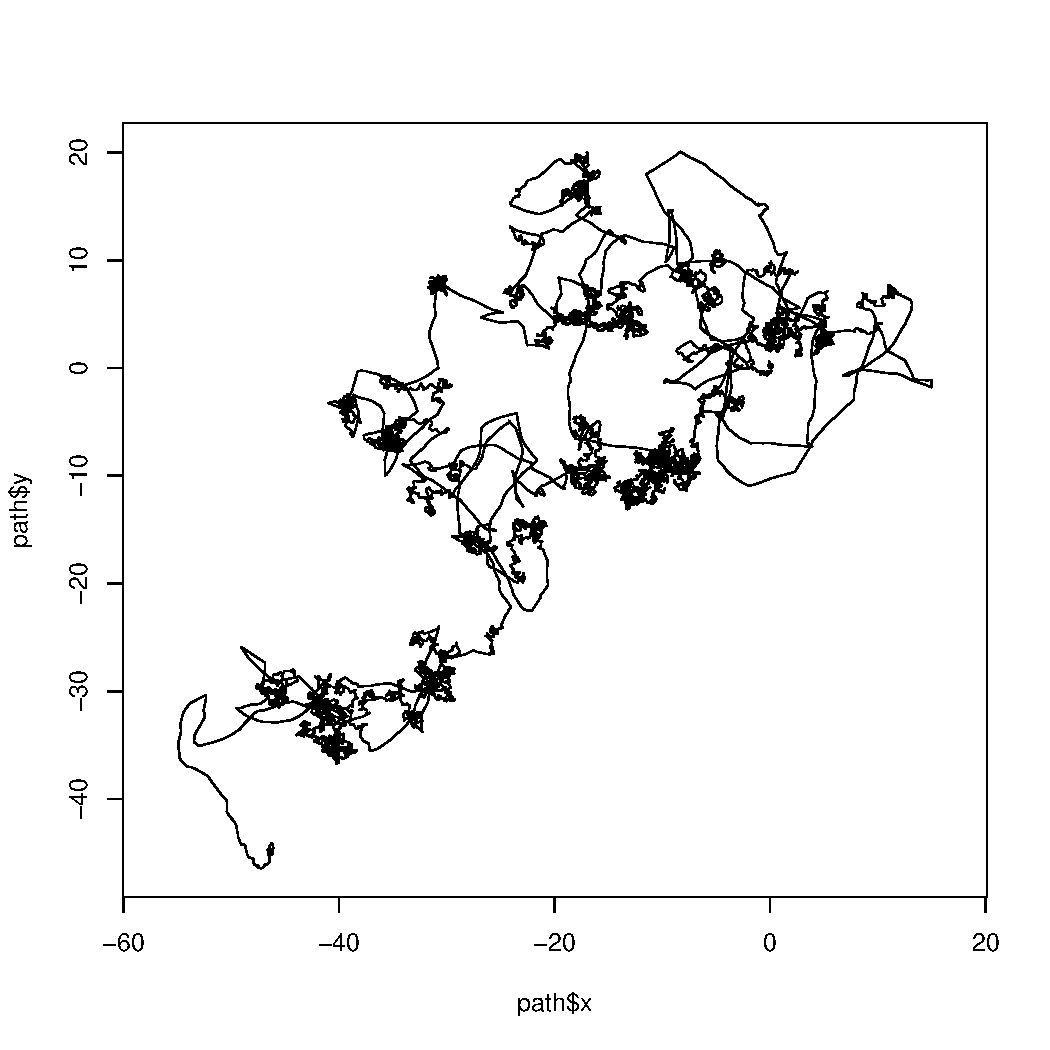
\includegraphics[scale=0.4]{pathPractical2-1.pdf}}
\only<2>{\includegraphics[scale=0.4]{pathPractical3-1.pdf}}
\end{column}
\end{columns}
\end{frame}



\subsection{Trajectories, a certain aspect of the movement}
\begin{frame}[fragile]{Effect of sampling step}

  \only<1>{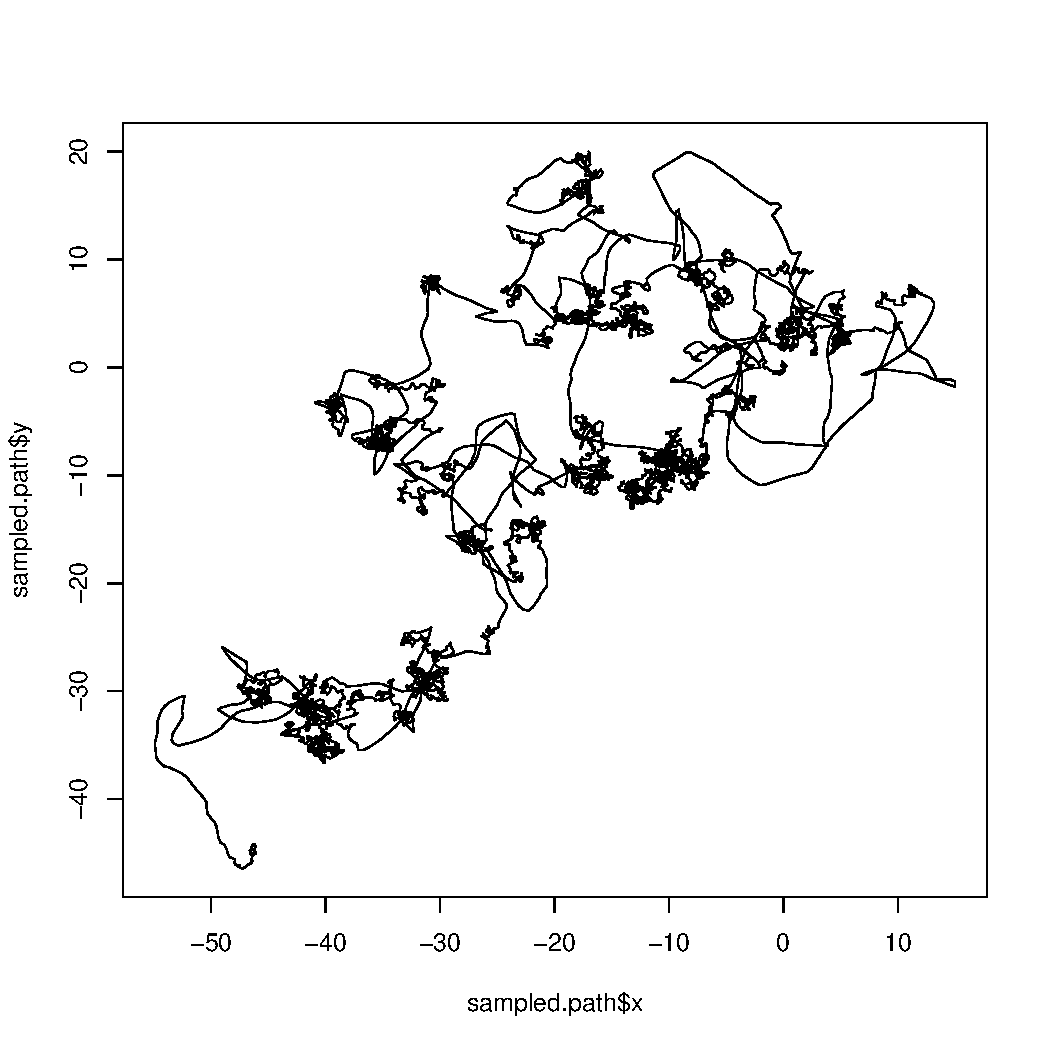
\includegraphics[scale=0.4]{pathPractical4-1.pdf}}
\only<2>{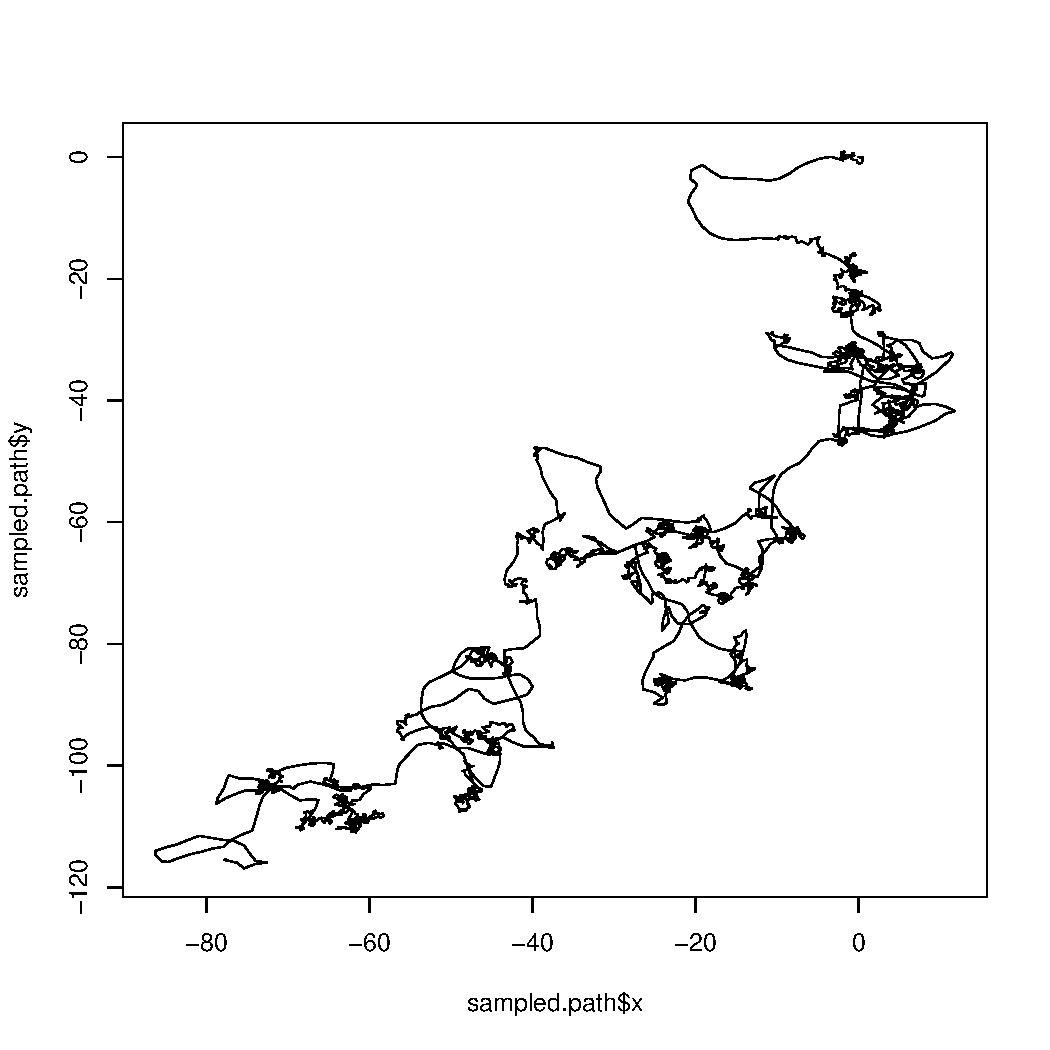
\includegraphics[scale=0.4]{pathPractical4-3.pdf}}
\only<3>{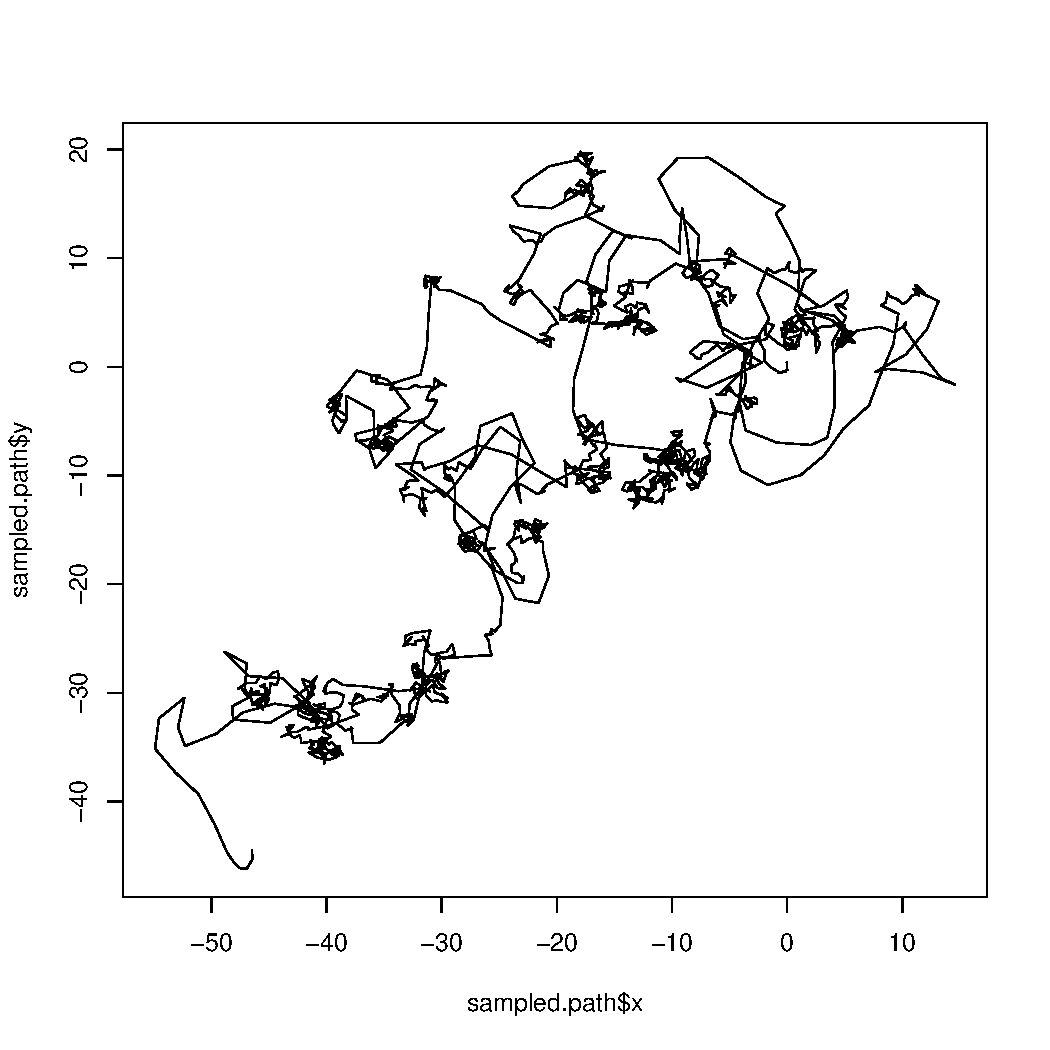
\includegraphics[scale=0.4]{pathPractical4-6.pdf}}
\only<4>{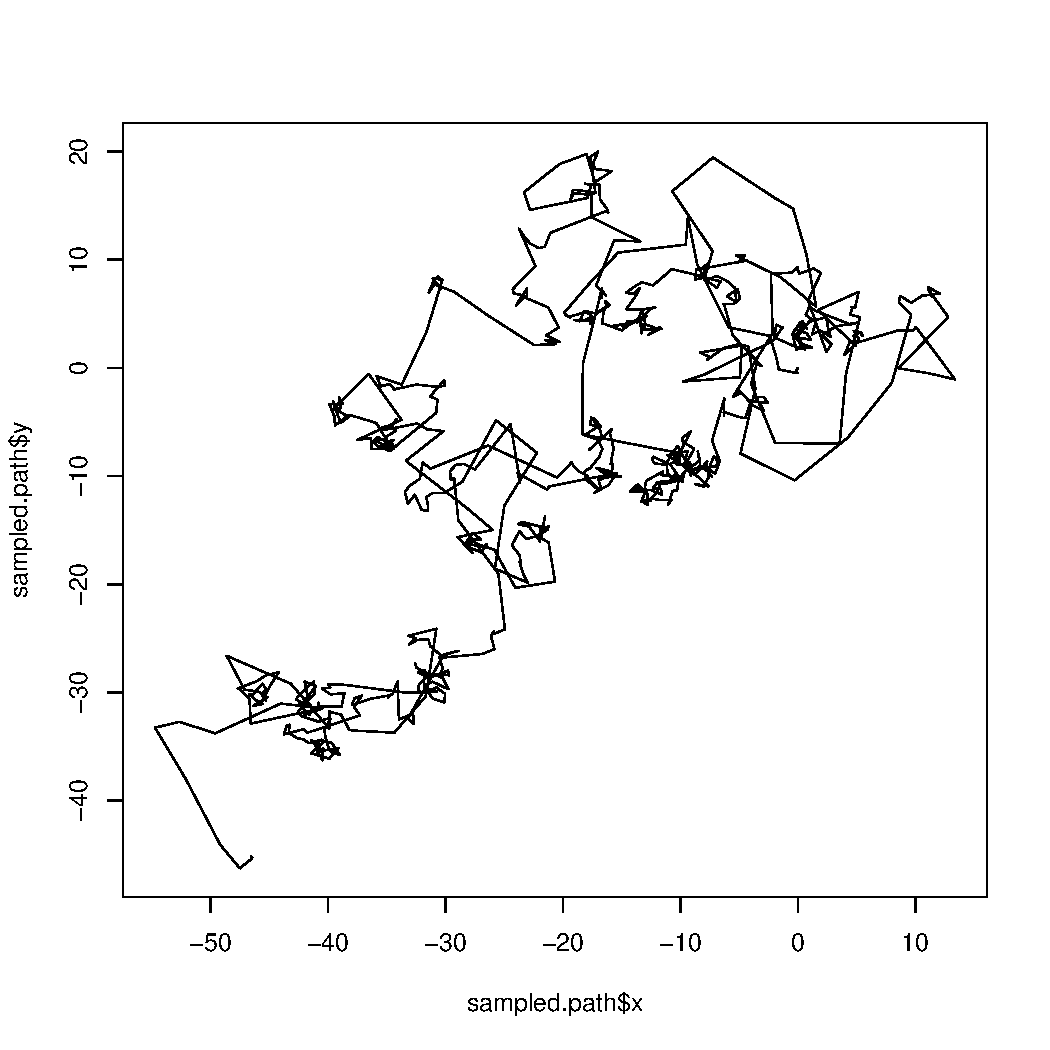
\includegraphics[scale=0.4]{pathPractical4-10.pdf}}
\only<5>{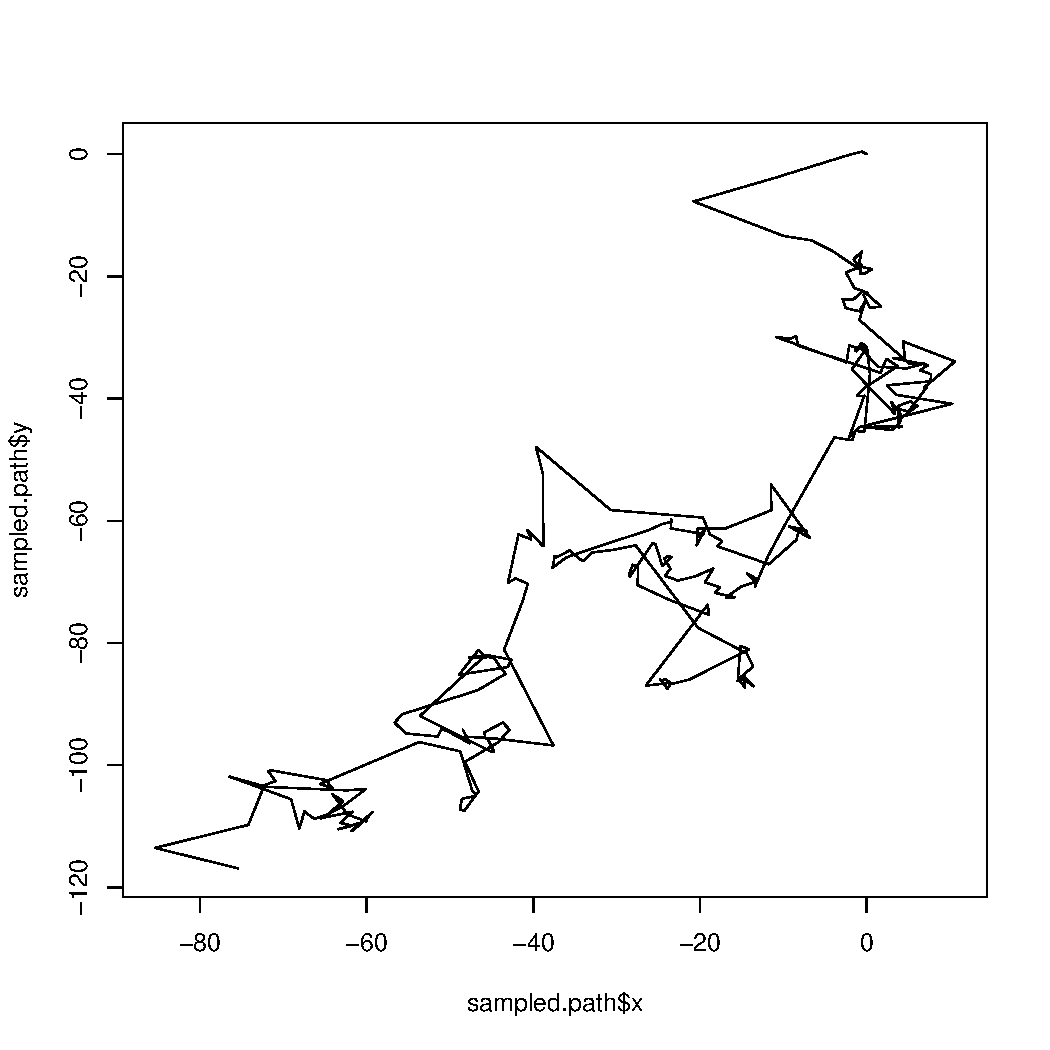
\includegraphics[scale=0.4]{pathPractical4-15.pdf}}

  \only<6>{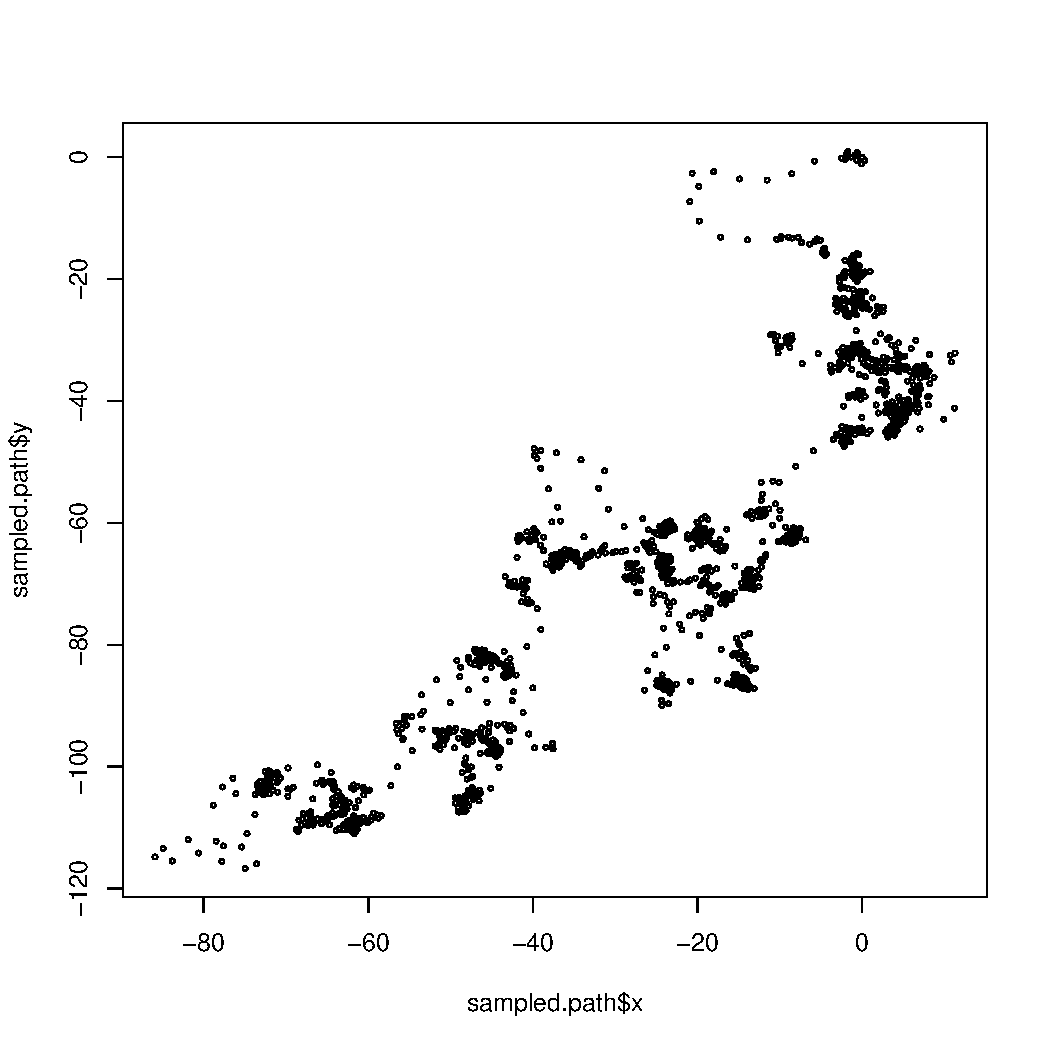
\includegraphics[scale=0.4]{pathPractical5-1.pdf}} 
\end{frame}


\begin{frame}{Summarising trajectories}
$(t_1, \ldots, t_N)$ denotes the time acquisition and $( (x_1,y_1),  \ldots, (x_N,y_N))$ the position at those times.

\only<1>{
  \paragraph{Trajetories as Turning angle and Speed}
  \begin{columns}
  \begin{column}{0.4\textwidth}
  
  $$\boldsymbol{\Phi}=(\phi_{2}, \ldots,\phi_{N})$$
    $$\boldsymbol{S}=(S_{2}, \ldots,\S_{N}),$$
    with $S_i=dist_i/(t_i-t_{i-1})$
    \end{column}
  \begin{column}{0.6\textwidth}
  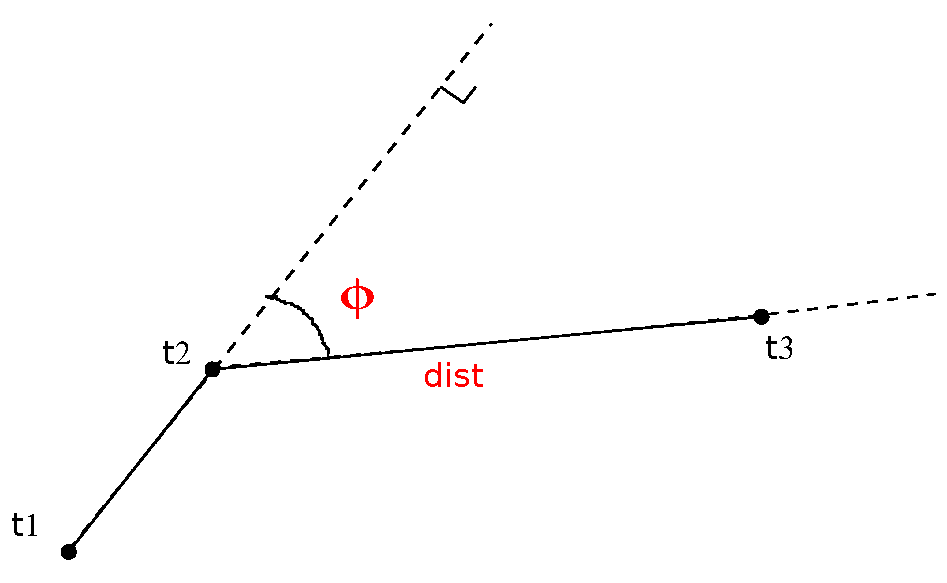
\includegraphics[scale=0.3]{Speed1.pdf}
  \end{column}
  \end{columns}
  $$ $$
}
\only<2>{
  \paragraph{Trajetories as Persistent and Normal Velocity}
  \begin{columns}
  \begin{column}{0.4\textwidth}
  
  $$\boldsymbol{V}^P=(V^P_{2}, \ldots,V^P_{N})$$
    $$\boldsymbol{V}^N=(V^N_{2}, \ldots,V^N_{N})$$
    with 
  \begin{align*}
  V^P_i&=S_i \, cos(\phi_i)\\
  V^N_i&=S_i \, sin(\phi_i)
  \end{align*}
  \end{column}
  \begin{column}{0.6\textwidth}
  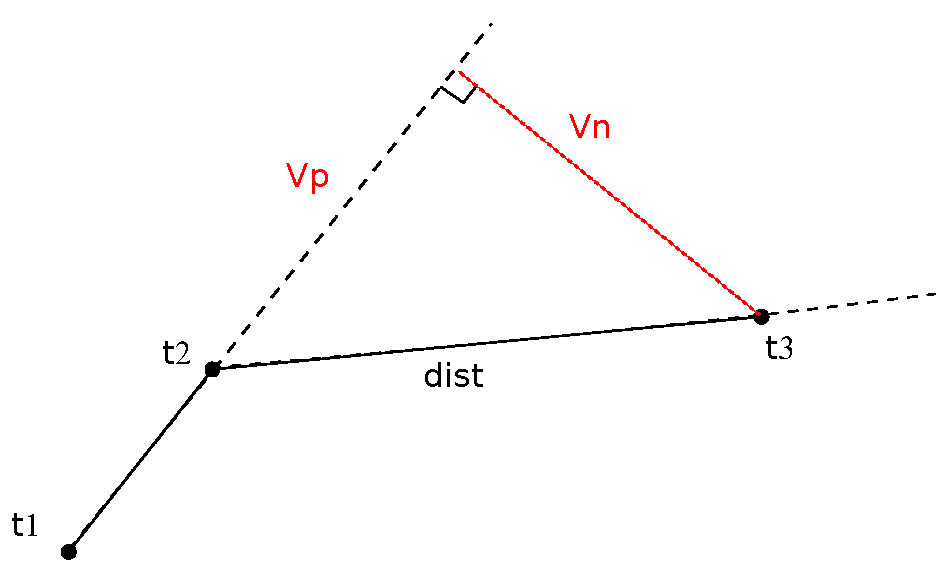
\includegraphics[scale=0.3]{Speed2.pdf}
  \end{column}
  \end{columns}
}
\end{frame}


\begin{frame}{Trajectories data}
\paragraph{How trajectories data migh be considered?}
\begin{itemize}
\item A sequence of (time, position)
\item Turning angle and speed sequences
\item Persistent and Normal Velocity sequences
\end{itemize}
\pause
\paragraph{What is affected by sampling?}
\begin{itemize}
\item A sequence of (time, position)
\item Turning angle and speed sequences
\item Persistent and Normal Velocity sequences
\end{itemize}
\pause
\paragraph{Model approach:}
\begin{itemize}
\item Most methods don't consider the two phenomena : movement and sampling process.
  \item Results will be closely dependent of the sampling step.
  \end{itemize}
\end{frame}

\subsection*{Convention}


\begin{frame}{Convention}
\paragraph{Notation:}
{\small
\begin{itemize}
\item $\Ybf = (Y_1, \ldots, Y_n) = $ observed data (typically Speed)
 \item $\Zbf $ unobserved data (typically State, for mixture  and Hidden Markov model)
 \item $\Thetabf$ = the unknown parameters of $\Ybf$ and $\Zbf$.
\end{itemize}
}
\paragraph{Graphical Representation (DAG):} 
\begin{columns}
\begin{column}{0.3\textwidth}
\centering{Change point}\smallskip
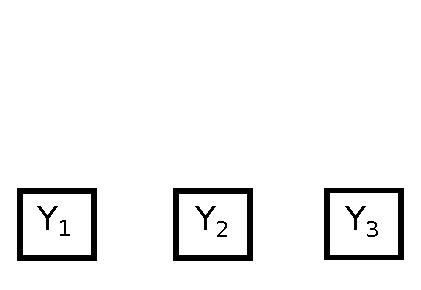
\includegraphics[scale=0.5]{Dag1.pdf}
\end{column}
\begin{column}{0.3\textwidth}
\centering{Mixture point}
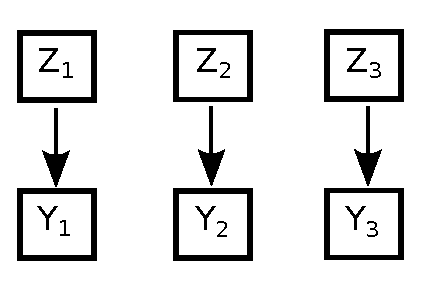
\includegraphics[scale=0.5]{Dag2.pdf}
\end{column}
\begin{column}{0.3\textwidth}
\centering{HMM}
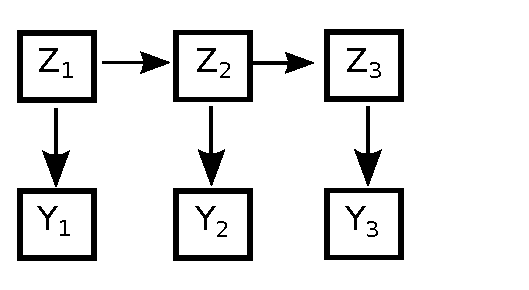
\includegraphics[scale=0.5]{Dag3.pdf}
\end{column}
\end{columns}
\end{frame}
%#show plan at the beginning of each secion except the first one
\AtBeginSection[]
{
 \begin{frame}<beamer>
 \frametitle{Plan}
 \tableofcontents[currentsection]
 \end{frame}
}

